\documentclass[english]{article}
\usepackage[T1]{fontenc}
%\usepackage[latin9]{inputenc}
\usepackage[utf8]{inputenc}
\usepackage{float}
\usepackage{graphicx}
\usepackage{babel}
\begin{document}

\section{Procesos}

Para implementar procesos inicialmente se decidió utilizar como base el código proveído por la cátedra. Luego de bastante tiempo sin llegar a nada, se decidió comenzar desde cero.

Se realizó un diagrama del stack necesario para un proceso resultando en el siguiente:

\begin{figure}[H]
\begin{center}
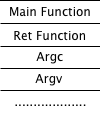
\includegraphics[width=5cm,height=2.5cm,keepaspectratio]{stack}

\caption{Stack frame}
\end{center}
\end{figure}

Una vez realizado ése diagrama, se procedió a armar manualmente el stack para correr el sistema operativo, haciendo que la función kmain sea solo una función dummy que llamase a una función de assembler para que crease dicho stack frame. Una vez construido éste, se cambió el ESP con otra función de assembler y el sistema siguió ejecutando en la función indicada por el stack frame.

Luego de entender como funciona el stack para ejecutar una función determinada, pasandole ciertos argumentos y haciendo que en su retorno, vaya a otra función, se procedió a crear una función que agregase éstos "procesos" a una lista para que luego puedan ser procesados por el scheduler.

\subsection{Scheduler}
Se decidió implementar un scheduler con prioridad, y un scheduler de tipo Round Robin.
Éste inicialmente se disparaba cada dos ticks, pero eso hacía el sistema muy lento.

\subsubsection{Scheduler con prioridad}
Al usar un scheduler con prioridad, los procesos pasan a ser más o menos importantes dependiendo de que prioridad se le asignó en su creación. Los procesos lanzados por el usuario mediante comandos en la consola son creados con una determinada prioridad. Hay un grupo de procesos que corre con prioridades especiales, uno de ellos el el proceso \emph{idle}.

Éste corre con prioridad muy baja, dado que es el que se ejecuta cuando no hay ningún otro proceso listo para ejecutarse. Otro grupo de procesos que corre con proridad especial son las shells.

Las shells no son bloqueantes, por lo que constantemente están polleando el tecleado para ver si hay nuevos caracteres que mostrar. Ésto hace que sea necesario hacer que las shells tengan distintas prioridades dependiendo de si están activas o no. La shell activa pasa a tener más de un 80\% del uso del procesador, y las restantes menos de un 5\%.

\subsection{Estados}
Cada proceso puede tener alguno de los siguientes estados:
\begin{itemize}
\item READY: El proceso está listo para ejecutarse
\item RUNNING: El proceso está siendo ejecutado en ese momento
\item CHILD\_WAIT: El proceso está bloqueado esperando que algún hijo finalice. Esto sucede cuando, por ejemplo, una consola ejecuta un proceso en \emph{foreground}.
\end{itemize}

\section{Driver disco ATA}

La implementación de driver $ATA$ que se utilizó en este $SO$ permite
acceso a un sector con offset y tamaño arbitrario (tanto para lectura
como para escritura). Si bien realizar esto, dificultó la programación
del driver, permite tener una lógica de programación mas simple en
las capas superiores ya que no es necesario leer un sector entero
para lugego ir hasta el offset deseado y obtener de ahi los bytes
necesarios (ni hablar si se quiere tomar información que se encuentra
partida en varios sectores contiguos). Es por eso que el driver utilizado
permite $"abstraerse"$ de esta división por sectores y poder acceder
a disco a partir de un sector con cualquier offset y cualquier cantidad
de bytes que se quiera leer.

La implementacion utilizada además presenta métodos para detección
de las propiedades de un disco (Si es removible, ATA, soporta DMA
y LBA), no se pudo (por falta de tiempo) crear un comando para listar
las cualidades de los discos conectados desde las consolas, pero se
espera poder mostrarlos para la próxima entrega.

Un detalle a mencionar es que la escritura al disco con un offset
es muy cara ya que ATA solo permite escribir de un sector entero,
por lo que para escribir una prte de uno de estos, primero hay que
leerlo entero en un buffer auxiliar, luego pisar los lugares a cambiar
y luego guardarlos, lo que seria equivalente a dos accesos a disco
solo para grabar una $x$ cantidad de bytes. Por lo que siempre se
intentará grabar la mayor cantidad de bytes posibles en cada acceso.

\pagebreak{}


\section{Disk Cache}

Debido a los problemas de eficiencia mencionados en la sección anterior,
se decidió que seria una buena idea tener una estructura cache, que
minimize los accesos a discos sin consumir mucha cantidad de memoria
ni procesamiento. 

La implementación de esta capa es muy sencilla, consiste en un vector
de $N$ estructuras en la que cada una tiene el contenido de un sector
entero y campos para indicar si el sector se encuentra sucio (si tiene
cambios con respecto al disco) y a que sector y disco corresponde.

El algoritmo de reemplazo elegido es el de LRU (es que menos accesos
tuvo, se reemplaza). 

Un problema al implementar esta capa era que hacer con los sectores
sucios ya que como se encuentran en RAM, hasta no ser guardados, la
información es propensa a perderse (ya sea por fallas del sistema,
corte de luz, etc). Frente a esto se decidió que cada una cantidad
fija de $ticks$, todos los sectores sucios serian escritos a disco. 

\pagebreak{}


\section{File System}

Nuestro File System se divide en dos partes, la primer parte es, el
file system en si y la segunda es la administración de la infomación
en el disco duro ($DiskManager$).

Para el manejo de archivos se decidió tomar la misma implementacion
que usa Linux. Es decir, archivos regulares, directorios, symbolic
links, etc son todos la misma estructura $fs$\_$node$ y lo único
que los diferencia es su campo $mask$ (en donde se define el tipo).
Inicialmente se comenzó tratando a cada tipo de archivo como un tipo
de estructura diferente, pero terminamos conluyendo que se volvía
muy compleja la logica de parseo de información en el disco.


\subsection{Manejo de disco}

Debido a la notable lentitud que posee el acceso a disco frente el
acceso a memoria, se diseñó el almacenamiento de la información dando
mas importancia siempre a la cantidad de accesos a disco por sobre
cantidad de bytes desperdiciados por archivo.

Uno de los primeros problemas que se presentaron al comenzar a trabajar
en disco, era como averiguar si un determinado sector de memoria era
o no valido. Frente a esto, en cada Header (mas adelante se hablara
mejor de estos) se agregó un campo $magic$ que sirve para la validacion
de los campos a leer. En otras palabras, si el magic number del header
leido coincide con el magic number definido en el SO, entonces exite
una estructura valida almacendada en esa posición de memoria. \\


El disco duro para este file system fue dividido básicamente en cuatro
partes:
\begin{enumerate}
\item File System header
\item Memory bitmap (bloques libres y ocupados en el disco)
\item Vector de iNodos
\item Archivos
\end{enumerate}

\begin{figure}[H]
\begin{center}
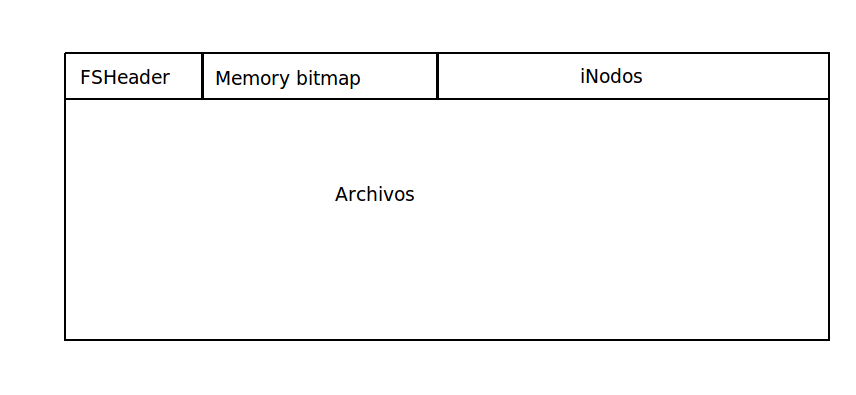
\includegraphics[width=10cm,height=5cm,keepaspectratio]{Imagen_disco}

\caption{Imágen disco duro}
\end{center}
\end{figure}


Para el F.S. Header simplemente se guardó un magic number y dos números
mas para indicar el tamaño máximo del vector de inodos y la cantidad
actual de inodos que se tienen guardados.

Cuando el SO se inicializa, intenta leer este sector de memoria, si
el magic number es valido, quiere decir que exite una particón valida
y entonces se intenta cargarla.

En cuanto al vector de iNodos, se trata de un vector de $N$ estructuras
de tamaño fijo (muy importante!) ya que permite el acceso al elemento
$i$ mediante una simple operacion matematica. En cada una de estas
estructiras del vector, se tiene almacenda una estructura de tipo
$DiskPage$, para indicar en que bloque del disco puede la informacion
ser encontrada y dos enteros: uno para indicar la cantidad de bloques
que esta página tiene reservada para su uso y otro para la cantiad
de bytes utlizados por el contenido del usuario.

La parte del disco dedicada a archivos se encuentra dividida en bloques
de tamaño fijo definido por el SO. Lo mas importante para destacar
en esta parte es la forma que se tiene para el almacenamiento de cada
archivo, el formato elejido para el almacenamiento de la información
es muy parecido al de una $LinkedList$. Todo archivo en disco consiste
de:
\begin{enumerate}
\item Disk Page
\item File Header
\item Su contenido
\end{enumerate}

\begin{figure}[H]
\begin{center}
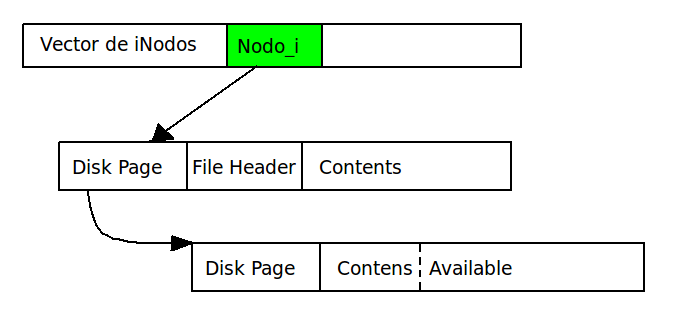
\includegraphics[width=10cm,height=7cm,keepaspectratio]{Archivo}

\caption{Formato de almacenamiento de un archivo}
\end{center}
\end{figure}


La estructura $File$$Header$ se guarda una única vez por cada archivo
y es la que posee el nombre, tipo, permisos y demás atributos que
no son parte del contenido en si.\\


El primer algorimto que se utilizó para reservar memoria para un archivo
consisitia en ir leyendo cada bloque del disco desde el principio
y utilizar apartir de ahi los que necesiten y esten diponibles. Inicialmente
parecia funcionar bien (ya que no se tenía mas de 2 o 3 archivos creados),
pero, a medida que se empezó a avanzar con el $SO$ y se requeria
de mayor catidad de archivos y carpetas, nos dimos cuenta de lo terriblemente
lento que se volvía este algoritmo. Luego se lo reemplazo por uno
que utiliza un $memory$ $bitmap$, el cual se encuentra junto al
FS header completando todo el primer sector del disco . Cada bit de
mapa, indica si el bloque $i$ de la parte de archivos se encuentra
ocupada o libre. De esta manera, reservar bloques sigue siendo$o(n)$
pero con la importantisima diferencia que solo se escribe cada sector
a utilizar y no se lee solamente uno solo (para escribir el header
del sector recien reservado) contra todos del anterior algoritmo.


\subsection{Manejo en RAM}

El manejo de inodos es ram es bastante sencillo, el $F.S.$ mantiene
un vector con los últimos inodos consultados y ofrece la interfaz
para el SO para la modificiacion y consulta de estos úlimos en disco.
Cada vez que un nuevo inodo es consultado, se toma la siguiente posicion
del vector y se carga allí la información de disco de este inodo para
luego retornarla.

Un detalle a tener en sobre esta implementación de $F.S.$, es que
no guarda ningún contenido de archivos (no cachea), ya que consideramos
que eso debe ser trabajo de una capa map entre el $diskManager$ y
el driver de disco ($diskCache$).

\pagebreak{}


\section{Problemas, posibles soluciones y features a agregar}
\begin{itemize}
\item File System:

\begin{itemize}
\item Cada vez que se crea un nuevo archivo, el FSHeader es consultado y
se incrementa el valor de la cantidad actual de inodos en el disco
y se utiliza este nuevo valor para utizar la siguiente posición del
vector de inodos (para el nuevo archivo). Se quiere aclarar que esta
es una implementación que nos parece muy mala y se tiene planeado
cambiarla por una en la que se utilize un bitmap, en donde el bit
$i-esimo$ indicaría si el sector esta libre o no (mismo algoritmo
utilizado para el manejo de espacio de archivos en el disco duro). 
\item Queda a implementar el comando borrar archivo, que esperamos este disponible
para la próxima entrega.
\end{itemize}
\item Otros

\begin{itemize}
\item Uno de los problemas mas importantes que tiene la actual versión del
$SO$ es la falta de semáforos y mutexs, especialmente para el momento
de reserva de memoria y para la lectura/escritura de archivos! (problema
de los N lectores y un escritor). Queda en la lista de cosas para
agregar en futuras actualizaciones del SO ya que no pudo ser implementad
por falta de tiempo.\end{itemize}
\end{itemize}

\end{document}
